\subsection{Signal conditioning on synthetic VEPs}
The VEP conditioning chain was verified on 150 seeded synthetic records (50 per class; 250\,Hz). The 50\,Hz response of the forward--backward notch is $-\notchDb$\,dB, the fitted 50\,Hz amplitude fell from \ampBefore{} to \ampAfter{} (mean reduction \nMainsDb\,dB, a lower bound set by the noise floor), and the P100 latency was recovered within one sample (4\,ms) in \nWithin{} of \nTrials{} records (Table~\ref{tab:p100}). A single-pass implementation of the same filters, with a group delay of \gdTen, \gdTwenty{} and \gdThirty\,ms at 10, 20 and 30\,Hz, was indistinguishable at this sampling rate, so the case for zero-phase processing rests on the principle that latency is the clinical quantity \cite{odom2016}, not on an empirical gain.

\begin{figure}[!t]
\centering
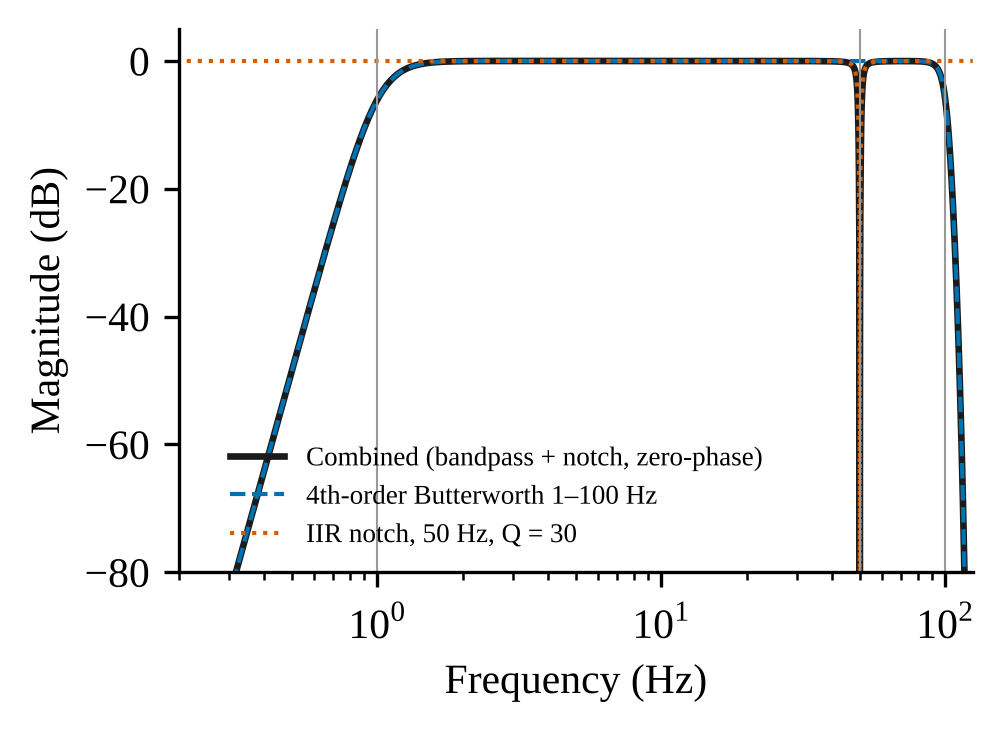
\includegraphics[width=\columnwidth]{figs/fig_filter_col.png}
\caption{Effective (forward--backward) magnitude response of the conditioning filters.}
\label{fig:filter}
\end{figure}

\begin{table}[!t]
\caption{Detected P100 latency in ms (mean $\pm$ SD over 50 synthetic trials per class).}
\label{tab:p100}
\centering\footnotesize
\begin{tabular}{@{}lcccc@{}}
\toprule
Class & True & Raw & Zero-phase & Single-pass\\
\midrule
Healthy Control & 100 & $101.8\pm2.3$ & $100.6\pm1.9$ & $101.1\pm1.8$ \\
Glaucoma & 108 & $107.4\pm2.7$ & $108.0\pm2.9$ & $108.2\pm2.3$ \\
Optic Neuritis/CVI & 140 & $141.3\pm2.5$ & $140.8\pm2.1$ & $141.0\pm2.7$
\\
\bottomrule
\end{tabular}
\end{table}

\subsection{Model size, cost and software verification}
The default three-class CAFN has \textbf{1{,}955{,}140} trainable parameters and 2.60\,G multiply--accumulates per sample at $64^3$ (0.39\,G at $32^3$) (Table~\ref{tab:params}); the 3D spatial encoder holds 46\% of the parameters and 97\% of the compute, the multi-scale temporal encoder 40\% of the parameters, and the gated bidirectional fusion 14\% of the parameters but under 0.5\% of the compute. The repository's automated suite now contains 340 tests (unit and integration, including end-to-end runs of the command-line tools, the cohort loaders and the experiment runner); all pass on macOS with Python 3.14, and on Ubuntu 22.04 with Python 3.12 and CUDA (one test is skipped on that host). Running on a second platform exposed three latent defects that the first platform had masked (a type annotation that fails on Python $\le$3.13, a device mismatch in the evaluation-only path on CUDA, and a unit test whose assertion was mathematically vacuous); all were fixed. The two real-file readers (CTF MEG and EDF polysomnography) were checked on real recordings, and the deterministic adaptive pooling was verified to match PyTorch's pooling in forward and backward passes.

\begin{table}[!t]
\caption{Trainable parameters and multiply--accumulates (M, at $64^3$) per component of the default CAFN.}
\label{tab:params}
\centering\footnotesize
\begin{tabular}{@{}lrr@{}}
\toprule
Component & Parameters & MACs (M)\\
\midrule
Spatial encoder (3D ResNet + SE) & 894{,}504 & 2522.68 \\
Temporal encoder (multi-scale 1D CNN) & 785{,}936 & 65.89 \\
Gated bidirectional fusion & 265{,}218 & 11.01 \\
Positional embeddings & 8{,}192 & 0.00 \\
Attention pool & 129 & 0.00 \\
Heads (3) & 1{,}161 & 0.00 \\
\midrule
Total & 1{,}955{,}140 & 2600 \\
\bottomrule
\end{tabular}
\end{table}
